% Paper 5, English edition. Chinese primary: paper_zh.tex.
% Build: tectonic paper_en.tex (offline: tectonic --only-cached paper_en.tex)
\documentclass[10pt]{article}
\usepackage[margin=1in]{geometry}
\usepackage{amsmath}
\usepackage{amssymb}
\usepackage{booktabs}
\usepackage{tabularx}
\usepackage{longtable}
\usepackage[numbers]{natbib}
\usepackage{tikz}
\usetikzlibrary{arrows.meta,positioning}
\usepackage[hidelinks]{hyperref}

\title{\textbf{Four Concepts, Four Types:\\Levels, Boundaries, and a Translation Protocol for\\Intelligence, Human Intelligence, Artificial Intelligence, and AGI}}
\author{Yugui Yu\\ YYG Strategy Lab\\ \texttt{they4897@gmail.com}}
\date{}

\begin{document}
\maketitle

\begin{abstract}
\noindent Intelligence, human intelligence, artificial intelligence, artificial general intelligence---four terms used daily across the literature, policy, and industry discourse, yet no authoritative account of their levels and boundaries exists: a single compilation collects some seventy informal definitions of intelligence; AGI definitions entered a period of institutionalized competition between 2023 and 2026, while industry systematically swaps words to avoid being bitten by its own definitions. This paper advances two theses. First (the typology): the four terms are not four rungs of one ladder but four different types of concepts---intelligence is a capacity concept, human intelligence a sample concept, artificial intelligence an artifact concept, and AGI a reference-frame concept; each type has a different form of ``completed definition,'' and the popular ``narrow--general--super'' ladder is a narrative device that strings four concept types on a single line. Second (the layered structure): within each concept one must distinguish the ontological layer (what it is), the epistemic layer (what evidence supports attributing it to a system), and the methodological layer (what procedure detects it); the chronic root of definitional disputes is three illicit slides---operationalism (measurement passing as definition), the mereological fallacy (mechanism passing as the location of a capacity), and criterion promotion (engineering criteria passing as conceptual content). The core contribution is a translation protocol: a table mapping engineering observations (circuits, features, gradients, benchmark scores) to the conceptual claims they license, each row with its conditions of validity, together with a catalogue of illicit translation forms. Under the protocol, claims of the form ``generalization is in the weights'' are not errors but overreaches: the attribution level of a capacity predicate is the combination of system and environment range, and a relational property has no location. The paper closes with the four terms' final positions in the human-referential theory of AGI, falsifiability clauses, and an appendix mapping the argument onto the Chinese-language context.
\end{abstract}

\medskip
\noindent\textbf{Keywords:} intelligence definitions; artificial general intelligence; construct validity; operationalism; mereological fallacy; mechanistic interpretability; conceptual levels; human-referential theory of AGI

\section{Introduction}\label{sec:intro}

The four terms are used daily in artificial-intelligence discourse, yet no consensus has ever formed on how they relate. The question ``what is intelligence?'' has had none since at least 1923\cite{boring1923intelligence}; the informal definitions compiled by Legg and Hutter number about seventy\cite{legg2007definitions}---the count has grown, not converged, over a century. ``What is artificial general intelligence?'' (AGI) compounds the same predicament: between 2023 and 2026, AGI definitions entered a period of institutionalized competition---performance-level matrices\cite{morris2023levels}, a psychometric model definition\cite{hendrycks2025definition}, and an economic-clause definition\cite{openai2018charter} coexist and conflict; meanwhile industry and regulatory discourse systematically swap words (frontier models, superintelligence, general-purpose AI), and no major institution is willing to be bound by its own five-year-old definition or to rule on whether AGI has been achieved. The only ``level diagram'' in wide circulation among the four terms---the three-rung ladder from narrow AI to AGI to superintelligence---is a popular convention, not a scholarly classification, and, as this paper argues, is itself a carrier of conceptual confusion.

Two kinds of everyday discourse make the absence of consensus conspicuous. The first comes from the definition side: many ``definitions'' are in fact measurement procedures. ``Intelligence as the tests test it''\cite{boring1923intelligence} is the prototype of this form; its contemporary variants include taking a measurement functional as the definition of intelligence\cite{legg2007universal}, an evaluation protocol as the definition of generality\cite{morris2023levels,chollet2019measure}, and an economic clause as the definition of AGI\cite{openai2018charter}. The second comes from the engineering side: mechanistic interpretability research observes structure in weights, circuits, and gradients, and in transmission these observations are promoted into assertions that ``generalization, intelligence, is in there.'' This paper's diagnosis of both kinds of discourse is the same: they are not false propositions but \emph{overreaching propositions}---claims legitimate within one layer, translated into another without passing any condition check. Herein lies the structural reason such claims fail to persuade: a proposition in which method passes for definition cannot be refuted---test failures can always be attributed to the method (benchmark contamination, distribution mismatch, too narrow a task set), and the ``definition'' itself is never injured. A proposition that never risks failure is not an epistemic claim; it is a creed.

This paper does three things. First, it organizes the four terms into four concept types and explains why each type's form of ``completed definition'' differs (Section~\ref{sec:types}). Second, it equips every concept with a three-layer structure---ontological, epistemic, methodological---and diagnoses existing definitional disputes as three illicit slides, resting the diagnosis on a catalogue of verbatim quotations (Section~\ref{sec:layers}). Third, it gives a translation protocol: a table from engineering observations to conceptual claims, with conditions of validity and a catalogue of illicit forms (Section~\ref{sec:protocol}); this is the paper's core contribution: it does not forbid cross-layer translation but requires every translation to present its conditions. Section~\ref{sec:program} places the four terms within the human-referential theory of AGI, Section~\ref{sec:falsify} states falsifiability clauses, Appendix~A gives the claim catalogue, and Appendix~B maps the argument onto the Chinese-language context.

The division of labor with the first three papers of this research program is explicit. The theory paper argued that generality is a relational property with respect to the open set of human practices\cite{yu2026theory}; this paper uses that result as the ready-made theoretical form of the reference-frame concept. The concept-unbundling paper separated the engineering goal of artificial intelligence from the machine mind\cite{yu2026twogoals}; this paper uses its ``functional intelligence'' as the criterion of the artifact concept. The methodology paper's disclosure audit\cite{yu2026methodology} serves here as an exemplar of correctly formed methodological-layer instruments. The incremental contribution of this paper---the typology of four terms, the three-layer structure, and the translation protocol---has, to the best of our literature search, no precedent (in either English- or Chinese-language literature; see the absence claims in Sections~\ref{sec:survey} and~\ref{sec:cn}).

\section{The State of the Definitions: Lineages and Drift}\label{sec:survey}

\subsection{Intelligence: A Century Without Consensus}

The two poles still cited in modern discussion took shape between 1904 and 1923. One pole is psychometrics: from the statistical fact that nearly all cognitive tests positively correlate, Spearman proposed the general factor $g$\cite{spearman1904general}, opening a measurement tradition that works quite well within human samples. The other pole is the operationalist stance: Boring's dictum that intelligence is what the tests test\cite{boring1923intelligence}---the definition is the measurement operation. After Bridgman proposed that a concept is a set of operations\cite{bridgman1927logic}, operationalism quickly receded in the physical sciences, yet it recurs throughout the history of intelligence definitions (Section~\ref{sec:layers}).

The formal tradition is represented by Legg and Hutter: ``Intelligence measures an agent's ability to achieve goals in a wide range of environments''\cite{legg2007universal}, given formal shape as a weighted expected reward over all computable environments. This path defines intelligence as a carrier-neutral measure of capacity, and human intelligence is demoted to a point on the scale. Against it, Chollet defines intelligence as ``the skill-acquisition efficiency'' of a system, given task scope, priors, and experience\cite{chollet2019measure}, and asserts that skills are merely fixed outputs of the intelligent process---there exists no task such that skill on that task alone suffices to demonstrate intelligence. The two definitions clash: the first would judge a system that ``bought a large stock of skills'' highly intelligent; the second judges it a fancy skill library. A century on, the shape of the disagreement has not converged; only the vocabulary has changed.

\subsection{Human Intelligence: Consensus Within a Sample}

For human intelligence, psychology in fact has a serviceable working consensus. The Cattell--Horn--Carroll three-stratum model organizes ability into a top stratum $g$, roughly ten broad abilities in the middle (fluid reasoning, crystallized knowledge, processing speed, working memory, among others), and dozens of narrow abilities at the base\cite{mcgrew2023chc}; contemporary mainstream intelligence tests are designed on this model. Two consensus documents supply the most-cited verbal definitions: the American Psychological Association task force report\cite{neisser1996intelligence} and ``Mainstream Science on Intelligence,'' signed by fifty-two researchers\cite{gottfredson1997mainstream}.

The boundary of this consensus is often ignored: it covers the Homo sapiens sample only. Most of the seventy-odd definitions compiled by Legg and Hutter come from psychologists working on human samples---``many definitions of intelligence are in fact definitions of human intelligence'' is not a rhetorical flourish but a fact verifiable directly from the compilation\cite{legg2007definitions}. Hern\'andez-Orallo's universal psychometrics argues systematically that tests calibrated on a human reference frame fail when extrapolated to machines and animals\cite{hernandezorallo2017measure}; Chollet adds an important reversal: a human-centered reference frame is ``not only legitimate but necessary''---because the technology serves humans---provided it is made explicit, with priors and developer injections counted into the measure\cite{chollet2019measure}. That is, the field has already acknowledged that the word ``intelligence'' oscillates between a human-centered and a carrier-neutral stance, but it has never organized this oscillation itself into a distinction of concept types. That is what this paper does.

\subsection{Artificial Intelligence: Defining the Making, Not the Intelligence}

The founding text of artificial intelligence deliberately bypasses the definition of intelligence. The programmatic sentence of the Dartmouth proposal is that every aspect of learning or any other feature of intelligence can in principle be so precisely described that a machine can be made to simulate it\cite{mccarthy1955dartmouth}---intelligence is an undefined primitive; what is defined is the making. McCarthy's own formal statement continues the structure: artificial intelligence is the science and engineering of making intelligent machines, especially intelligent computer programs\cite{mccarthy2007whatis}. The textbook tradition arranges the space of definitions into the four-cell matrix ``thinking humanly/thinking rationally/acting humanly/acting rationally'' and selects the rational-acting branch\cite{russell2021aima}; the Turing-test line sets the human as the indistinguishable counterpart\cite{turing1950computing}.

This making-first structure has a famous back door: since intelligence itself is undefined, the boundary of ``artificial intelligence'' can only move with engineering achievement---Tesler's theorem, ``AI is whatever hasn't been done yet''\cite{tesler1997effect}, characterizes exactly this negative, moving category. It explains why McCarthy's definition is compatible with any concrete technology, and it foreshadows the third slide diagnosed in Section~\ref{sec:layers}: when engineering criteria (benchmarks, products, commercial success) grow strong enough, they come to be taken, unnoticed, as definitions of intelligence itself.

\subsection{Artificial General Intelligence: A Period of Institutionalized Competition}

Before 2023 the AGI definition lineage was a minor academic tradition: Legg and Hutter's definition is the same as that of intelligence\cite{legg2007universal}; Goertzel phrased it as ``the ability to achieve complex goals in complex environments''\cite{goertzel2014agi}. From 2023 it enters institutionalized competition: the GPT-4 ``sparks'' paper works with an implicit definition of broad cognitive ability\cite{bubeck2023sparks}; DeepMind's leveled framework gives a ``performance $\times$ generality'' matrix, operationalizing ``general'' as ``the range of tasks at which target performance thresholds are met'' and rating current frontier models as ``emerging AGI''\cite{morris2023levels}; the OpenAI charter gives the economic definition---``highly autonomous systems that outperform humans at most economically valuable work''\cite{openai2018charter}; in 2025, a definition co-signed by thirty-three authors takes the Cattell--Horn--Carroll psychometric model as its skeleton, defining AGI as ``matching the cognitive versatility and proficiency of a well-educated adult''\cite{hendrycks2025definition}. On the critical side, it has been argued that AGI discourse's definitions ``embrace a series of incompatible values and assumptions''\cite{blili2024unsocial,blili2025stop}; on the measurement side, new proposals keep arriving\cite{xu2024meant,dhar2025generality,gignac2024defining}.

Over the same period a twofold word drift occurred: product and regulatory language moved from AGI to ``frontier models'' and ``general-purpose AI'' (the latter presuming systemic risk from training-compute thresholds); laboratory narratives moved from AGI to ``superintelligence.'' The definitional disagreement was set aside by swapping words, not resolved.

\subsection{The Chinese-Language Context}\label{sec:cn}

The Chinese-language context offers two angles of observation unavailable in English.

The first is a history of terminological division of labor. Since Lu Zhiwei's first revision of the Binet scales in 1924\cite{zhang2020psychometrics}, psychology has fixed on \emph{zhili} (智力, ``intelligence'') for its tests and quotients; the translation \emph{rendong zhineng} (人工智能, ``artificial intelligence'') entered in the late 1970s and was formally adopted in the early 1980s, fixing on \emph{zhineng} (智能, ``intelligent capability''). The disciplinary split between \emph{zhili} and \emph{zhineng} persists to this day, supplemented at the popular-science level by a three-tier progression of \emph{zhili} (base layer) $\to$ \emph{zhineng} (application layer) $\to$ \emph{zhihui} (智慧, ``wisdom,'' value layer)---but this three-tier frame has never received rigorous conceptual analysis. In other words, the Chinese context has long held an intuition about levels of ``intelligence''; what it has lacked is a scholarly level diagram.

The second is drift in policy vocabulary. The 2017 New-Generation AI Development Plan mentions ``general artificial intelligence'' only within its basic-theory layout\cite{state2017plan}; Beijing's 2023 municipal policy operationally equates general artificial intelligence with ``a general large-model technology system''\cite{beijing2023measures}---a visible gap from scholarly definitions (e.g., Zhu Song-Chun's team's three characters---infinite tasks, self-defined tasks, value-driven---and the TongTest system\cite{zhu2025tongtest}); central documents, exemplified by the 2025 Government Work Report, avoid ``general artificial intelligence'' entirely, preferring policy coinages such as ``AI+,'' ``embodied intelligence,'' and ``intelligent economy''\cite{gov2025report}. The domestic definitional lineage is its own tradition: Zhang Bo's three-generations account periodizes ``specialized--general''\cite{zhang2020third}; Zhong Yixin's mechanism approach gives an originally Chinese definition via information--knowledge--intelligence conversion\cite{zhong2018mechanism}; on the philosophical side, Liu Yongmou argues that AGI is caught in a nominalist predicament---there exist concrete AGI projects, yet no agreed definition of AGI\cite{liu2024complex}; Zhao Tingyang and Yin Jie approach from the dimension of subjectivity\cite{zhao2019selfconscious}. To the best of our literature search, no systematic analysis of the levels and boundaries of the four terms appears in the Chinese-language literature (Appendix~B locates the interlocutors and states the absence claim).

\subsection{Summary: The Vacancy at the Levels}

Taken together: ``intelligence'' has two mutually exclusive definitional traditions; ``human intelligence'' has an in-sample consensus that is often passed off as the general definition; ``artificial intelligence'' deliberately does not define intelligence, only the making; ``AGI'' is in a period of institutionalized definitional competition and evades adjudication by word-swapping. No authoritative account of the four terms' level relations exists; generality has four mutually incompatible operationalizations (task range, environmental openness, skill-acquisition efficiency, autonomy level); and human intelligence plays four roles in AI definitions (reference frame, counterpart, economic accounting unit, criticized yardstick). The vacancy is not a shortage of literature; it is the lack of a framework that can say clearly \emph{which kind of concept each of the four terms is}. Section~\ref{sec:types} supplies it.

\section{Thesis One: Four Terms, Four Concept Types}\label{sec:types}

\subsection{The Criterion}

The classificatory criterion is this: a concept's type is fixed by the form of its success criterion---what ``the definition question has been answered'' means for it. Under this criterion the four terms fall into four types (Figure~\ref{fig:matrix}).

\begin{figure}[t]
\centering
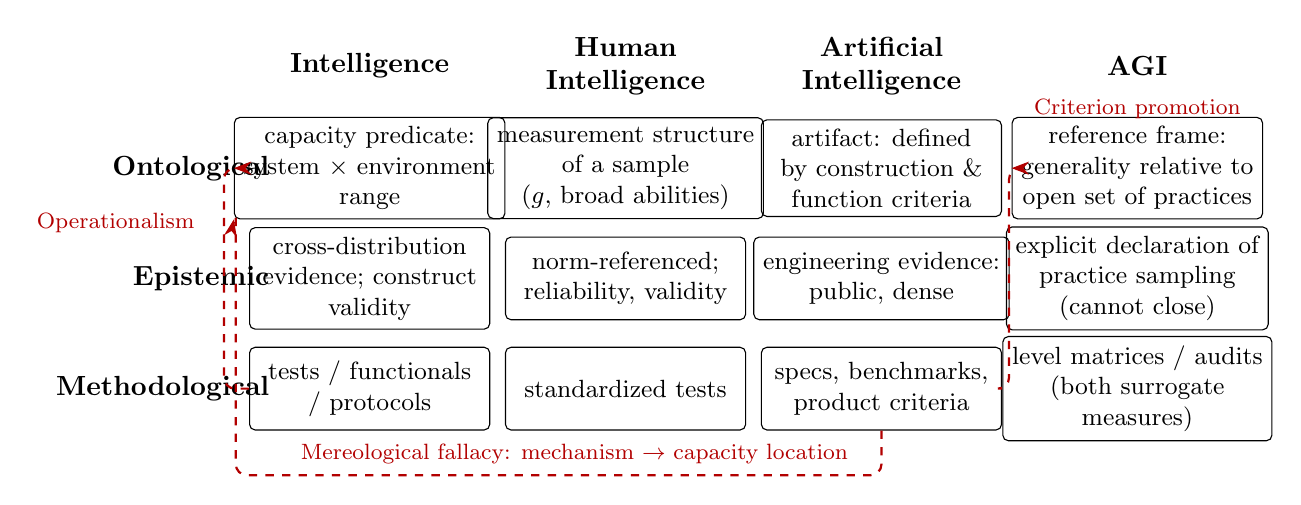
\begin{tikzpicture}[font=\small,
  box/.style={draw, rounded corners=2pt, minimum width=3.05cm, minimum height=1.05cm, align=center},
  slide/.style={-{Stealth[length=2.2mm]}, dashed, thick, red!70!black}]
% layer labels
\node[anchor=east, font=\bfseries] (ont) at (0.75,4.2) {Ontological};
\node[anchor=east, font=\bfseries] (epi) at (0.75,2.8) {Epistemic};
\node[anchor=east, font=\bfseries] (met) at (0.75,1.4) {Methodological};
% column labels
\node[font=\bfseries] at (1.9,5.5) {Intelligence};
\node[font=\bfseries, align=center] at (5.15,5.5) {Human\\Intelligence};
\node[font=\bfseries, align=center] at (8.4,5.5) {Artificial\\Intelligence};
\node[font=\bfseries] at (11.65,5.5) {AGI};
% intelligence column
\node[box] (i1) at (1.9,4.2) {capacity predicate:\\system $\times$ environment\\range};
\node[box] (i2) at (1.9,2.8) {cross-distribution\\evidence; construct\\validity};
\node[box] (i3) at (1.9,1.4) {tests / functionals\\/ protocols};
% human intelligence column
\node[box] (h1) at (5.15,4.2) {measurement structure\\of a sample\\($g$, broad abilities)};
\node[box] (h2) at (5.15,2.8) {norm-referenced;\\reliability, validity};
\node[box] (h3) at (5.15,1.4) {standardized tests};
% AI column
\node[box] (a1) at (8.4,4.2) {artifact: defined\\by construction \&\\function criteria};
\node[box] (a2) at (8.4,2.8) {engineering evidence:\\public, dense};
\node[box] (a3) at (8.4,1.4) {specs, benchmarks,\\product criteria};
% AGI column
\node[box] (g1) at (11.65,4.2) {reference frame:\\generality relative to\\open set of practices};
\node[box] (g2) at (11.65,2.8) {explicit declaration of\\practice sampling\\(cannot close)};
\node[box] (g3) at (11.65,1.4) {level matrices / audits\\(both surrogate\\measures)};
% three slide arrows (orthogonal routing along margins and column gaps)
\draw[slide, rounded corners=4pt] (i3.west) -- (0.05,1.4) -- (0.05,4.2) -- (i1.west);
\node[font=\footnotesize, red!70!black, anchor=east] at (-0.2,3.5) {Operationalism};
\draw[slide, rounded corners=4pt] (a3.south) -- (8.4,0.3) -- (0.2,0.3) -- (0.2,3.675) -- (i1.south west);
\node[font=\footnotesize, red!70!black] at (4.5,0.57) {Mereological fallacy: mechanism $\to$ capacity location};
\draw[slide, rounded corners=4pt] (a3.east) -- (10.02,1.4) -- (10.02,4.2) -- (g1.west);
\node[font=\footnotesize, red!70!black] at (11.65,4.95) {Criterion promotion};
\end{tikzpicture}
\caption{Four concepts $\times$ three layers. Columns are concept types (capacity, sample, artifact, reference frame); rows are layers (ontological, epistemic, methodological). Red dashed arrows mark the three illicit slides diagnosed in Section~\ref{sec:layers}: methodological-layer claims promoted to ontological-layer definitions (operationalism); engineering observations promoted to the location of a capacity (mereological fallacy); artifact criteria promoted to capacity definitions and reference-frame content (criterion promotion).}
\label{fig:matrix}
\end{figure}

\subsection{Intelligence: A Capacity Concept}

The attribution level of the ``intelligence'' predicate is \emph{the combination of system and environment}: to say a system is intelligent is always relative to a range of environments. Legg and Hutter's formal definition states this mathematically---intelligence is expected performance over a space of environments\cite{legg2007universal}; psychometrics does the same by restriction to the population of tasks humans encounter. The common point: the success criterion of intelligence takes the form of a \emph{measurement}---the definition question is answered when there exists a measurement with a construct-validity claim. As a capacity concept, intelligence does not answer ``what is the system made of''; it answers ``what can the system do, within what range.''

\subsection{Human Intelligence: A Sample Concept}

``Human intelligence'' is not another capacity; it is \emph{the measurement structure of a tested population}. Its success criterion takes the form of norms: the definition question is answered when, for a defined population, there exist standardized instruments, norms, and reliability-and-validity evidence\cite{spearman1904general,mcgrew2023chc,neisser1996intelligence}. The relation of sample concept to capacity concept is projection, not subset: human intelligence is the projection of the intelligence concept onto the Homo sapiens sample, carrying a population boundary---which explains two things from Section~\ref{sec:survey}: why the psychometric consensus cannot be extrapolated to machines (the projection changed samples)\cite{hernandezorallo2017measure}, and why ``many definitions of intelligence are in fact definitions of human intelligence'' (the projection was mistaken for the preimage).

\subsection{Artificial Intelligence: An Artifact Concept}

``Artificial intelligence'' is an artifact: a class of engineering objects defined by construction and function criteria. Its success criterion takes the engineering form---functional specifications met, publicly checkable performance---and does not require ``possessing intelligence'' as a condition of membership. A search engine is artificial intelligence, regardless of whether anyone intends to award it the predicate ``intelligent.'' The concept-unbundling paper of this program has supplied the content of this layer: the engineering goal of artificial intelligence is functional intelligence in service of human practice, with public, dense, continuously improving success criteria\cite{yu2026twogoals}. The decisive consequence lies in the word ``artifact'': the criteria of an artifact concept (how well it works) do \emph{not} define the content of a capacity concept (what intelligence is)---this consequence becomes the diagnostic basis of the third slide in Section~\ref{sec:layers}.

\subsection{Artificial General Intelligence: A Reference-Frame Concept}

The type of ``AGI'' is the most counterintuitive: it is not a bigger capacity but a \emph{reference frame}. The theory paper has argued its form: generality is not a self-sufficient intrinsic property but a relational one---a system counts as ``general'' only relative to the open set of human practices it references; ``general'' refers to the openness of the practice set, ``high'' refers to the performance of human practitioners, and both are stipulations made on the demand side\cite{yu2026theory}. The success criterion of a reference-frame concept cannot close: it cannot be ``defined-complete'' by a specification; it can only be given as an explicit declaration---declaring which practice set is referenced and by what sampling it is approximated. This is the structural reason definitional disagreement cannot end: every AGI definition is in effect declaring a reference frame (the CHC ability inventory\cite{hendrycks2025definition}, the economically valuable work set\cite{openai2018charter}, the task-breadth threshold\cite{morris2023levels}), and disagreements between reference frames are not empirical disagreements; no experiment can adjudicate them.

\subsection{Against the Ladder: Four Relations Instead}

The popular three-rung ladder (narrow AI $\to$ AGI $\to$ superintelligence) strings the four concept types on a single univariate line, as if an ``intelligence quantity'' grew along the rungs. On the typology, the correct picture is four concepts plus four relations: human intelligence is the projection of intelligence onto the human sample (the measurement relation); artificial intelligence is the artifact class of candidate realizers of intelligence (the realization relation); performance evaluation of artificial intelligence calls on human intelligence as its baseline (the reference relation); AGI is the naming of the reference frame itself (the normative relation). The ladder is not wholly wrong; it is a category splicing: it welds ``the quantity of capacity'' (the vertical axis from first rung to third), ``the norms of the sample'' (humans on the middle rung), ``the criteria of the artifact'' (what counts as narrow), and ``the openness of the reference frame'' (what counts as general) onto one line. The resulting ``progress'' narrative---systems climbing the ladder---is precisely the progress-transfer illusion diagnosed by the concept-unbundling paper, transposed onto the level diagram\cite{yu2026twogoals}.

\subsection{The Form of ``Completed Definition'' for Each Type}

The typology yields a direct corollary table: a capacity concept may close with an operational definition, provided a construct-validity claim is attached (otherwise it degenerates into operationalism); a sample concept closes with norms; an artifact concept closes with a functional specification; a reference-frame concept \emph{never} closes with a definition---only with a declaration of the referenced set. The four forms of completion are not interchangeable: ``completing'' a capacity concept with an artifact specification (the third slide), or ``completing'' the ontological layer with a measurement (the first slide), are type mismatches. This corollary table also explains every phenomenon of the AGI definitional competition (Section~\ref{sec:survey}): each competitor answers another type's question with one type's form of completed definition.

\section{Thesis Two: Three Layers and Three Illicit Slides}\label{sec:layers}

\subsection{The Three-Layer Frame}

For each concept, distinguish three kinds of claims: the \textbf{ontological layer} (what it is---claims of existence and attribution), the \textbf{epistemic layer} (what evidence supports ``some system has it''---claims of evidence and inference), and the \textbf{methodological layer} (what procedure detects it---claims of operations and protocols). The three layers are not three ways of saying the same thing: they differ in truth conditions, in modes of failure, and in the cost of revision. Chinese philosophical discourse has a stable, textbook-level usage of the ontology--epistemology--methodology trichotomy; this paper adopts it directly and constrains every ``$X$ is in layer $Y$'' assertion within its layer.

The matrix of Figure~\ref{fig:matrix} is the working diagram of this paper. The chronic knot of definitional disputes appears in it as three cross-layer slides.

\subsection{Slide One: Operationalism---Measurement Passing as Definition}

The operationalist thesis that a concept is a set of operations\cite{bridgman1927logic} has receded in the physical sciences; psychometrics paid that price first: tests do measure something, but the test itself cannot say what---Cronbach and Meehl invented ``construct validity'' and the ``nomological network'' to remedy exactly this\cite{cronbach1955construct}. In the history of AI definitions the lesson has replayed three times. First: a measurement functional (expected reward over a space of environments) taken as the definition of intelligence\cite{legg2007universal}. Second: an evaluation protocol (skill-acquisition efficiency; level matrices) taken as the definition of generality\cite{chollet2019measure,morris2023levels}. Third: an economic clause taken as the definition of AGI\cite{openai2018charter}.

One terminological distinction first. ``Operationalizing'' in the leveled framework's title\cite{morris2023levels} is the neutral usage of evaluation engineering---translating abstract goals into measurable indicators. The operationalism criticized here is Bridgman's---taking the measurement operation as the \emph{entire content} of the concept. The former is necessary; the latter overreaches. The boundary between them is precisely the epistemic layer: evaluation engineering stays in the methodological layer and submits evidence upward to the epistemic layer; operationalism skips the epistemic layer and answers an ontological question directly with a methodological claim.

The structural defect of operationalist definitions is irrefutability. Test failures can always be attributed to the method---benchmark contamination\cite{zhang2024gsm1k}, choice of metric\cite{schaeffer2023mirage}, too narrow a task set---while the ``definition'' itself is never injured. A proposition that bears no risk of failure is not an epistemic claim. This also explains the intuition from the introduction: definitions that pass methodology off as epistemology fail to persuade because creeds do not enter empirical wagers.

The turn came in 2021--2025: measurement theory is entering AI evaluation in an institutionalized way---construct-validity critiques of benchmarks\cite{raji2021benchmark}, the demonstration that ``emergence'' is a metric artifact\cite{schaeffer2023mirage}, overfitting exposed by cloned benchmarks\cite{zhang2024gsm1k}, up to the 2025 wave of papers formally importing psychometric validity frameworks into LLM evaluation\cite{bean2025measuring,salaudeen2025measurement,wallach2024evaluating,jo2025benchmark,xiao2023metriceval}. This line offers the most direct support to this paper, but it all stops at the ``evaluation--capability'' link; a systematic diagnosis that pushes the validity critique up to the ``definition'' layer we could not find in the literature---that vacancy is where this paper stands. The nearest philosophical precursor is the diagnosis of ``AI operationalism''\cite{mussgnug2024operationalism}, which argues that machine-learning practice equates concepts with their operationalizations, thereby ``temporarily fixing reference.'' This paper runs in the opposite direction: not to describe the phenomenon but to supply the layered rules and the translation protocol that prevent it.

\subsection{Slide Two: The Mereological Fallacy---Mechanism Passing as the Location of Capacity}

The second slide occurs on the engineering side. Bennett and Hacker's ``mereological fallacy'' diagnoses the attribution of whole-level predicates to parts---the category mistake of ``the brain thinks''\cite{bennett2003philosophical}. The diagnosis has been imported into AI discussions of semantic attribution of the ``the model is thinking'' kind\cite{vantill2024personification,helliwell2024wittgenstein}, but not yet applied to the level confusion between capacity discourse and evaluation scores---this paper takes that step.

The argument has three steps. First, the attribution level of a capacity predicate is the combination of system and environment range (Section~\ref{sec:types})---the subject of ``the system has capacity $C$ within environment range $E$'' is always the system, never weights, circuits, or gradients. Second, generality is a relational property\cite{yu2026theory}, and relational properties have no location: to say ``generalization is in the weights'' is not to err but to treat an unleavable property as locatable---like saying that weight is located in kilograms. Third, the legitimate products of mechanistic interpretability are \emph{mechanism attributions} and \emph{realization evidence}: finding the realizing mechanism of a capacity is not finding that capacity a residence---the realizer carries dispositions, dispositions hold relative to task distributions, and the attribution of capacity remains at the system level.

To avoid criticizing strengthened versions that exist only in retellings, the diagnosis rests on verbatim quotations, graded by assertion strength (full list in Appendix~A). Program level: ``Features are the fundamental unit of neural networks''\cite{olah2020zoomin}---offered as a speculative claim, asserting the fundamental unit of \emph{explanation} in the weights, not yet the location of capacity. Causal level: induction heads as ``the primary source of in-context learning'' in two-layer attention-only models\cite{olsson2022induction}---a mechanism attribution supported within its bounds by ablation evidence; legitimate, though the same paper's abstract is far more cautious---``preliminary and indirect evidence for a hypothesis.'' Implementation level: ``We fully reverse engineer the algorithm learned by these networks,'' with ``circuit formation'' among the three phases\cite{nanda2023progress}---the most literal version, holding for toy tasks. License level: ``attribution graphs provide hypotheses about mechanisms''; ``existence proofs''\cite{lindsey2025biology}---the authors restrict their own claims to the epistemic layer. Descriptive level: ``this concept universe has interesting structure at three levels''\cite{tegmark2024geometry}---a geometric observation making no conceptual claim.

Beyond the spectrum lies \emph{drift}. The same institution's paper says ``we cannot use attribution graphs to draw conclusions with certainty about the underlying model''\cite{lindsey2025biology}; its public-facing blog says ``we found that Claude plans ahead''\cite{anthropic2025thoughts}---across title, body, and transmission, assertion strength scales up step by step; community retellings then strip the hedges, turning ``might be the mechanism'' into ``is the mechanism.'' On the empirical side, counterexamples already exist: function-vector heads, not induction heads, dominate in-context learning in larger models\cite{yin2025which}; sparse autoencoders find no canonical units of analysis\cite{leask2025canonical}; cross-layer features drift across versions with circuit effectiveness falling in step\cite{anthropic2024crosscoders}; high probe accuracy does not entail structure in representations\cite{hewitt2019designing,belinkov2022probing}; subspace patching can manufacture an ``interpretability illusion''\cite{makelov2023illusion}; causal-probing methods trade completeness against selectivity\cite{canby2024reliable}. On the philosophical side, work on mechanistic explanation has begun: linking uncertainty matters more than transparency\cite{sullivan2022understanding}; levels of transparency distinguished\cite{creel2022transparency}; strategies of mechanism discovery normalized\cite{kastner2024explaining}; ``mechanistic interpretability needs philosophy''\cite{williams2025philosophy}; a mathematical philosophy of explanation\cite{ayonrinde2025mathematical}; and, nearest to this paper, ``causal claims must disclose identification assumptions''\cite{lin2026disclose}. But each covers one corner---single empirical counterexamples, limits of probing, causal identification---no one has given a layered diagnosis of the \emph{inference form} itself: ``structure observed $\to$ capacity resides therein.''

\subsection{Slide Three: Criterion Promotion---Artifact Criteria Passing as Capacity Definitions}

The back door of the third slide stands open in the founding texts: the making-first definitional structure of artificial intelligence (Section~\ref{sec:survey}) leaves intelligence as an undefined primitive. Engineering thereby gains a legitimate space: do not define intelligence; deliver function. But when an artifact's engineering criteria grow strong enough---benchmark wins, product success, economic returns---the criteria spill out of the artifact layer and are taken for the content of capacity concepts and even of the reference-frame concept: benchmark scores read as ``intelligence level,'' economic substitution read as ``generality achieved''\cite{openai2018charter}. The difference from slide one lies in the carrier: slide one is ``measurement passing as definition''; slide three is ``engineering goals passing as conceptual content''; the former occurs on the theoretical side of concepts, the latter on the applied side. They share the same gap---skipping the epistemic layer: between benchmark score and capacity claim, a construct-validity claim is missing\cite{raji2021benchmark,bean2025measuring}; between economic substitution and generality claim, a practice-sampling declaration is missing\cite{yu2026theory}.

\section{The Translation Protocol}\label{sec:protocol}

\subsection{Why a Protocol}

Cross-layer translation is not intrinsically illegitimate. Engineering observations must be able to enter conceptual discussion---otherwise interpretability research and evaluation science both lose their point; conceptual discussion must also be able to constrain engineering---otherwise definitional disputes are merely an academic game. The problem is that translation currently happens \emph{implicitly}. The most mature case is the 2025 CHC definition\cite{hendrycks2025definition}: it in fact completed a translation from a psychometric model to the AGI concept, yet with no explicit translation methodology---the reader cannot see which psychological constraints were carried in and which discarded. The purpose of the protocol is not to forbid translation but to make every translation \emph{show its conditions}. It upgrades the terminology table of this program's methodology paper into a methodology\cite{yu2026methodology}: that paper mapped words to words across communities (``rollout'' to ``practice-stream telemetry''); this paper maps propositions to propositions across layers---engineering observation statements to conceptual claims, with conditions of validity and a catalogue of illicit forms.

\subsection{The Translation Table}

Table~\ref{tab:protocol} is the protocol proper: six common kinds of engineering observation, the conceptual claim each licenses, and the conditions under which the translation holds.

\begin{table}[t]
\centering
\caption{The translation protocol: conditions of validity for engineering-observation $\to$ conceptual-claim translation.}
\label{tab:protocol}
\small
\begin{tabularx}{\textwidth}{p{3.6cm} X p{4.2cm}}
\toprule
Engineering observation & Licensed conceptual claim & Conditions of validity \\
\midrule
Performance on task $T$ drops after ablating circuit $c$ & $c$ is a contributing mechanism of the system on $T$ (methodological-layer claim) & The completeness--selectivity trade-off of the intervention is reported\cite{canby2024reliable}; causal identification assumptions are disclosed\cite{lin2026disclose} \\
A probe decodes feature $f$ from representations & Decodable information about $f$ exists in the representations & Control-task selectivity checks pass\cite{hewitt2019designing}; decoding is not use (amnesic probing)\cite{belinkov2022probing} \\
Geometric structure appears in feature space (leaves, crystals, directions) & The feature space has descriptive structure (descriptive level) & Stability of the structure is checked across training seeds and dictionary sizes\cite{leask2025canonical}; must not be translated as ``concepts live here'' \\
The model scores $S$ on benchmark $B$ & Relative to $B$'s task distribution, the system performs at $S$ & $B$ carries a construct-validity claim (what it measures) and a contamination check\cite{bean2025measuring,zhang2024gsm1k}; must not be translated as ``intelligence is $S$'' \\
The system reaches human level on a set $W$ of economically valuable tasks & Substitution evidence on $W$ (epistemic layer) & $W$ is explicitly declared as a sample of the open set of human practices\cite{yu2026theory}; the sampling is auditable\cite{yu2026methodology} \\
A phase transition occurs in training (e.g., grokking\cite{power2022grokking}) & A stage transition in training dynamics & Metric stability of the transition is checked\cite{schaeffer2023mirage}; must not be auto-translated as ``generalization has formed in the weights''\cite{nanda2023progress} \\
\bottomrule
\end{tabularx}
\end{table}

Every row shares three general rules. First, \emph{attribution preservation}: after translation the subject remains the system (or the combination of system and environment range)---never weights, circuits, gradients. Second, \emph{conditions travel}: when a claim leaves the methodological layer, its conditions of validity leave with it; an unconditional conceptual claim is an overreaching claim. Third, \emph{layer placement}: the product of translation must be marked with its layer---methodological-layer claims (mechanism, information), epistemic-layer claims (evidence, substitution), ontological-layer claims (only when all conditions are met and construct validity holds).

\subsection{A Catalogue of Illicit Translations}

Against the table, four recurrent illicit forms. \textbf{Locational} (``intelligence/generalization is in $X$''): assigning a position to a relational property---mereological fallacy. \textbf{Part-whole misattribution} (predicates of the system level attributed to components): wrong attribution level. \textbf{Promotion} (``score $S$'' $\to$ ``intelligence is $S$''; ``passes protocol $P$'' $\to$ ``the definition is $P$''): skipping construct validity---operationalism. \textbf{Universalization} (leaping from the tested distribution to the open set): skipping the sampling declaration---mistaking the projection for the preimage. The catalogue matches the table row by row: every illicit form is some licensed translation with its conditions of validity stripped away.

\subsection{A Corollary for AGI Definitions: Writing Definitions in Three Layers}

The protocol's corollary for the definition side: a responsible AGI definition should be written in three layers, not one sentence. Ontological: generality as a relational property with respect to which practice set (the reference-frame declaration)\cite{yu2026theory}; epistemic: what evidence counts as ``attainment''---task sets, population baselines, time windows (the epistemic declaration)\cite{morris2023levels,hendrycks2025definition}; methodological: what procedure measures it, how sampling is declared, what the failure conditions are (the methodological declaration)\cite{salaudeen2025measurement,yu2026methodology}. Reread this way: the level matrix is solid epistemic- and methodological-layer work that answers an ontological question under the name of ``operationalizing''\cite{morris2023levels}; the CHC definition is a serious ontological-layer declaration that does not declare the boundary of its sample projection (CHC is the sample structure of human intelligence, Section~\ref{sec:types}); the economic definition is a methodological-layer contract taken as an ontological verdict\cite{openai2018charter}. Three-layer writing does not dissolve definitional disagreement---disagreements between reference frames have no experimental adjudication---but it makes every disagreement fall in its own layer: nameable, comparable, retractable.

\section{Position in the Human-Referential Theory of AGI}\label{sec:program}

The final picture of the four terms takes its place in the human-referential theory of AGI and supports it in return. The theory paper argues: AGI is a reference-frame concept (generality relative to the open set of human practices); its means of realization is the fitting of practice; its normative position is that of an augmenting tool\cite{yu2026theory}. This paper completes its conceptual foundation: intelligence, as a capacity concept, is relational because capacity is defined jointly by the object of fitting and the range of practice---in its genesis, such intelligence is acquired by fitting practice\cite{yu2026theory}; human intelligence, as a sample concept, is the measurement face of the human reference frame in the theory; artificial intelligence, as an artifact concept, has its criterion (functional intelligence in service of human practice) fixed by the concept-unbundling paper\cite{yu2026twogoals}---and that paper's ``asymmetry of evaluation'' (public criteria on the capacity side, no consensus test on the mind side) receives its explanation in this paper's layered structure: capacity predicates have both a determinate system-level attribution and ready-made construct-validity procedures, whereas predicates of mind lack third-person tests; hence the two tracks diverge. The methodology paper's disclosure audit\cite{yu2026methodology} exemplifies the correct form of the methodological layer: it does not announce that generality was measured; it declares, for the sampling and cell-by-cell evidence disclosed by eight pipelines, exactly what is and is not claimed---conditions traveling with the translation.

The final placement in one sentence: \textbf{intelligence asks for measurement; human intelligence asks for norms; artificial intelligence asks for artifact criteria; AGI asks for a reference frame.} The four questions cannot stand in for one another, just as the four concepts do not lie on one ladder.

\section{Falsifiability Clauses}\label{sec:falsify}

Each of the three claims can be defeated. \textbf{Typology}: if future work shows that the four terms can be meaningfully measured by a single yardstick---one measure with undistorted predictive power simultaneously over the capacity structure of intelligence, the norms of human intelligence, the engineering criteria of artificial intelligence, and the reference set of AGI---then the four types merge, and the typology degenerates into a redundant classification; the literature providing that measure supersedes this paper. \textbf{Layered structure}: if some class of capacity predicates can be legitimately attributed to components---that is, a rigorous definition of ``component-level capacity'' with criteria undisturbed by counterexamples exists---then the mereological-fallacy diagnosis fails, and ``generalization is in the weights'' is promoted from overreach to testable claim; if mechanistic interpretability reaches that point, this paper becomes a superseded precursor. \textbf{Translation protocol}: if any of the four illicit forms proves reliable under declarable conditions (locational form for some locatable subclass of relational properties, or promotion form on some self-calibrating benchmark), the corresponding row of the catalogue is withdrawn and the table extended---the protocol carries its own revision clause. The absence claim is falsifiable in the same way: if any literature in English or Chinese already gives a systematic analysis of the four terms' levels and boundaries (under ``concept types'' or an equivalent frame), this paper's incremental-contribution claim is withdrawn in favor of citation.

\section{Conclusion}

Four terms, four concept types, three layers, one protocol. The diagnosis: a century of non-converging intelligence definitions, AGI definitions evading adjudication by word-swapping, engineering discourse installing intelligence into weights, public discourse failing to persuade---these are four manifestations of one structural defect: conceptual claims sliding between types and layers without presenting conditions. The typology returns the four terms to their seats; the layered structure gives each seat its truth conditions; the translation protocol sets checkpoints between the seats---not to close the border, but to check credentials. For engineering, the protocol's yield is more honest strong claims: mechanism attributions, existence proofs, in-distribution dispositions---each worth doing and worth saying, none of them a residence for capacity. For the definition side, the yield is three-layer writing: reference-frame declaration, epistemic declaration, methodological declaration---each in its layer, each staking its own falsification. For the Chinese-language context, the paper supplies the diagram that has been missing: the intuitive \emph{zhili--zhineng--zhihui} layering finally gains a scholarly form in concept types. In the end, the four terms take their places in the human-referential theory of AGI: intelligence is the capacity acquired by fitting practice; human intelligence is the measurement face of the reference frame; artificial intelligence is the artifact that carries the fitting; and AGI is that reference frame itself---measured against the open set of human practices, never to close.

\bibliographystyle{unsrtnat}
\bibliography{references_en}

\appendix

\section{Claim Catalogue: Verbatim Quotations and Assertion Strength}\label{app:catalog}

This catalogue collects the verbatim quotations on which the diagnosis rests, in two panels: the definition side (objects of the operationalism and criterion-promotion diagnoses) and the mechanism side (objects of the mereological-fallacy diagnosis). ``Source level'' marks the discourse level at which the quotation sits; ``strength'' is this paper's grading (program, causal, implementation, license, descriptive, transmission); ``licenses'' states what claim the quotation can support under the protocol of Section~\ref{sec:protocol}.

\subsection{Definition Side}

\begin{longtable}{p{3.4cm} p{4.6cm} p{1.6cm} p{1.6cm} p{3.4cm}}
\toprule
Source & Quotation & Source level & Strength & Licenses \\
\midrule
\endhead
Boring 1923\cite{boring1923intelligence} & ``Intelligence as the tests test it'' & Title & Operationalist prototype & Historical object of diagnosis only \\
Legg \& Hutter 2007\cite{legg2007universal} & ``Intelligence measures an agent's ability to achieve goals in a wide range of environments'' & Body & Definition level & Methodological-layer functional with conditions; not an ontological definition \\
Chollet 2019\cite{chollet2019measure} & Intelligence is ``the skill-acquisition efficiency'' of a system & Abstract & Definition level & Methodological-layer protocol, with priors declared \\
Morris et al.\ 2023\cite{morris2023levels} & ``at least as capable as a human at most tasks'' & Body & Epistemic-layer framework & A leveling artifact; no ontological verdict \\
OpenAI Charter\cite{openai2018charter} & ``highly autonomous systems that outperform humans at most economically valuable work'' & Policy text & Methodological-layer contract & Economic-substitution evidence; not attainment of generality \\
Hendrycks et al.\ 2025\cite{hendrycks2025definition} & ``matching the cognitive versatility and proficiency of a well-educated adult'' & Abstract & Ontological-layer declaration & A reference-frame declaration; sample-boundary declaration missing \\
Tesler's theorem\cite{tesler1997effect} & ``AI is whatever hasn't been done yet'' & Essay & Negative category & Historical footnote to the moving boundary \\
\bottomrule
\end{longtable}

\subsection{Mechanism Side}

\begin{longtable}{p{3.2cm} p{4.8cm} p{1.7cm} p{1.5cm} p{3.0cm}}
\toprule
Source & Quotation & Source level & Strength & Licenses \\
\midrule
\endhead
Olah et al.\ 2020\cite{olah2020zoomin} & ``Features are the fundamental unit of neural networks'' & Body & Program level & Program for units of explanation; not a location of capacity \\
Olsson et al.\ 2022 (abstract)\cite{olsson2022induction} & ``preliminary and indirect evidence for a hypothesis that induction heads might constitute the mechanism'' & Abstract & License level & Hypothesis-level evidence claim (compliant exemplar) \\
Olsson et al.\ 2022 (body)\cite{olsson2022induction} & induction heads ``appear to be the primary source of in-context learning'' (two-layer attention-only models) & Body (bounded scope) & Causal level & Mechanism attribution within bounds \\
Nanda et al.\ 2023\cite{nanda2023progress} & ``We fully reverse engineer the algorithm learned by these networks''; ``circuit formation'' among three phases & Abstract & Implementation level & Implementation evidence on toy tasks \\
Varma et al.\ 2023\cite{varma2023circuit} & grokking occurs when the task admits a generalising and a memorising solution & Abstract & Causal level & Mechanism account of a synthetic setting \\
Wang et al.\ 2024\cite{wang2024grokked} & ``the formation of the generalizing circuit'' & Abstract & Implementation level & Training-dynamics claim \\
Lindsey et al.\ 2025 (body)\cite{lindsey2025biology} & ``attribution graphs provide hypotheses about mechanisms''; ``existence proofs'' & Body & License level & Epistemic self-restriction (compliant exemplar) \\
Anthropic blog 2025\cite{anthropic2025thoughts} & ``we found that Claude plans ahead'' & Institutional blog & Transmission level & Strong transmission-layer claim (object of diagnosis) \\
Tegmark group 2025\cite{tegmark2024geometry} & ``this concept universe has interesting structure at three levels'' & Abstract & Descriptive level & Geometric description; no conceptual assertion \\
Park et al.\ 2024\cite{park2024linear} & ``high-level concepts are represented linearly as directions'' & Abstract (informal statement) & Hypothesis level & Formalized hypothesis with evidence \\
Gurnee \& Tegmark 2024\cite{gurnee2024space} & Title asserts ``Represent''; abstract eases to ``suggest $\ldots$ basic ingredients of a world model'' & Title/abstract & Title strong, abstract weak & A drift exemplar \\
Yin \& Steinhardt 2025\cite{yin2025which} & in-context learning depends primarily on function-vector heads, not induction heads & Abstract & Empirical counterexample & A counterexample to the strong reading \\
Leask et al.\ 2025\cite{leask2025canonical} & sparse autoencoders do not find canonical units of analysis & Title & Empirical counterexample & Evidence of non-canonical features \\
\bottomrule
\end{longtable}

How to read the list: the first eight mechanism rows form the strength spectrum ``program $\to$ causal $\to$ implementation $\to$ license $\to$ transmission''; the last five rows are descriptive-level, hypothesis-level, title--body drift exemplars, and empirical counterexamples.

\section{Mapping onto the Chinese-Language Context}\label{app:cn}

\subsection{A Timeline of the Terminology}

1922--1924: the Binet scales, revised, enter China; psychometrics fixes \emph{zhili} (智力). 1978--1981: the translation \emph{rendong zhineng} (人工智能) is adopted in mainland scholarship; the Chinese Association for Artificial Intelligence is founded. 2002--2003: Peking University establishes China's first department of intelligence science. 2022: the Ministry of Education lists ``Intelligence Science and Technology'' as a first-level discipline. The division of labor between \emph{zhili} (psychology) and \emph{zhineng} (intelligence science) persists today.

\subsection{Policy Vocabulary}

The details appear in Section~\ref{sec:cn}; the essentials: the 2017 plan mentions ``general artificial intelligence'' only in basic-theory layout\cite{state2017plan}; Beijing's 2023 policy equates it with a general large-model technology system\cite{beijing2023measures}; central documents, exemplified by the 2025 Government Work Report, shift to ``AI+,'' ``embodied intelligence,'' and ``intelligent economy'' without using the term\cite{gov2025report}. The drift of policy language is isomorphic to the international word-swap (frontier models, superintelligence): operational vocabulary routes around the definitional dispute.

\subsection{Locating the Interlocutors}

Zhu Song-Chun's team's three characters---infinite tasks, self-defined tasks, value-driven---and the TongTest\cite{zhu2025tongtest,zhu2023origin,zhu2025moment} form the strongest AGI definition system in the Chinese context; on this paper's layers, an ontological-layer declaration with epistemic-layer artifacts. Liu Yongmou's ``nominalist predicament''\cite{liu2024complex} is the meta-critique from Chinese philosophy; this paper's typology is a structural response to it (the predicament arises from demanding that four concept types share one form of ``completed definition''). Zhang Bo's three generations\cite{zhang2020third} and Tan Tieniu's official definitional formula\cite{tan2024lecture} supply the periodization and the policy baseline sentence. Zhong Yixin's mechanism approach\cite{zhong2018mechanism} gives an information-theoretic definition of intelligence whose terms ``ontological information/epistemic information'' resonate with this paper's three layers. Zhao Tingyang's ``new subject'' question, raised from the dimension of subjectivity\cite{zhao2019selfconscious}, falls in this framework on the normative face of the reference-frame concept. Absence claim: a systematic analysis of the four terms' levels and boundaries does not appear in the Chinese-language literature; should one exist, this paper defers to it and withdraws the claim.

\end{document}
